\begin{enumerate}[label=\alph*)]
  \item Pour construire la matrice
  
        \begin{equation*}
          A = \begin{bmatrix}
                1 & \textbf{1}^{\top}   \\
                \textbf{1} & -I_{n - 1}
              \end{bmatrix}
        \end{equation*}
        
        on utilise en \textsc{MATLAB} les commandes suivantes
        
\begin{verbatim}
n = 1000;
a11 = 1;
a12 = ones(1, n-1);
a21 = ones(n-1, 1);
a22 = -eye(n-1,n-1);
A = [a11,a12;a21,a22];
\end{verbatim}

      Ensuite, pour calculer la factorisation $LU$, on utilise la commande :
      
\begin{verbatim}
[L,U,P] = lu(A);
\end{verbatim}

  \item Pour visualiser la structure des facteurs $L$ et $U$, on écrit
  
\begin{verbatim}
figure(1)
spy(L)
figure(2)
spy(U)
\end{verbatim}  

    On voit sur la Figure \ref{fig:lu} que les facteurs sont pleins :

    \begin{figure}[h!]
      \begin{subfigure}[b]{0.5\linewidth}
        \centering
        \includegraphics[scale=0.4]{s4/matlab/L-eps-converted-to.pdf} 
        %\caption{Interpolation of $f$ using NCS \\ with $8+2$ points} 
        %\label{fig:q11_n8} 
      \end{subfigure}
      \begin{subfigure}[b]{0.5\linewidth}
        \centering
        \includegraphics[scale=0.4]{s4/matlab/U-eps-converted-to.pdf} 
        %\caption{Interpolation of $f$ using NCS \\ with $8+2$ points} 
        %\label{fig:q11_n8} 
      \end{subfigure} 
      \caption{Structure des matrices $L$ (à gauche) et $U$ (à droite) telles que $A = LU$.}
      \label{fig:lu}
    \end{figure}   
    
  \item On peut permuter la première ligne de $A$ avec la dernière, ainsi que la première colonne de $A$ avec la dernière, en utilisant la matrice de permutation $P$ donnée par
  
  
  \begin{equation*}
    P = \begin{bmatrix}
      0       & 0       & \dots   & 0       & 1 \\
      0       & 1       & \dots   & 0       & 0 \\
      \vdots  & \vdots  & \ddots  & \vdots  & \vdots \\
      0       & 0       & \dots   & 1       & 0 \\
      1       & 0       & \dots   & 0       & 0
        \end{bmatrix}
        ,
  \end{equation*}
  
  et en exécutant le produit $\tilde{A} = PAP$ : 
  
\begin{verbatim}
P = zeros(n,n);
P(1, n) = 1;
P(n, 1) = 1;
P(2:n-1, 2:n-1) = eye(n-2,n-2);
tildeA = P*A*P;
\end{verbatim} 

  \item La factorisation $LU$ de $\tilde{A}$, telle que $\tilde{A} = \tilde{L} \tilde{U}$ , ainsi que les structures des matrices $\tilde{L}$ et $\tilde{U}$, sont données par :
  
\begin{verbatim}
[tildeL, tildeU] = lu(tildeA);
figure(3)
spy(tildeL)
figure(4)
spy(tildeU)
\end{verbatim} 
    
   On trouve les structures pésentées dans la Figure \ref{fig:tildelu}.
   
   \begin{figure}[h!]
     \begin{subfigure}[b]{0.5\linewidth}
       \centering
       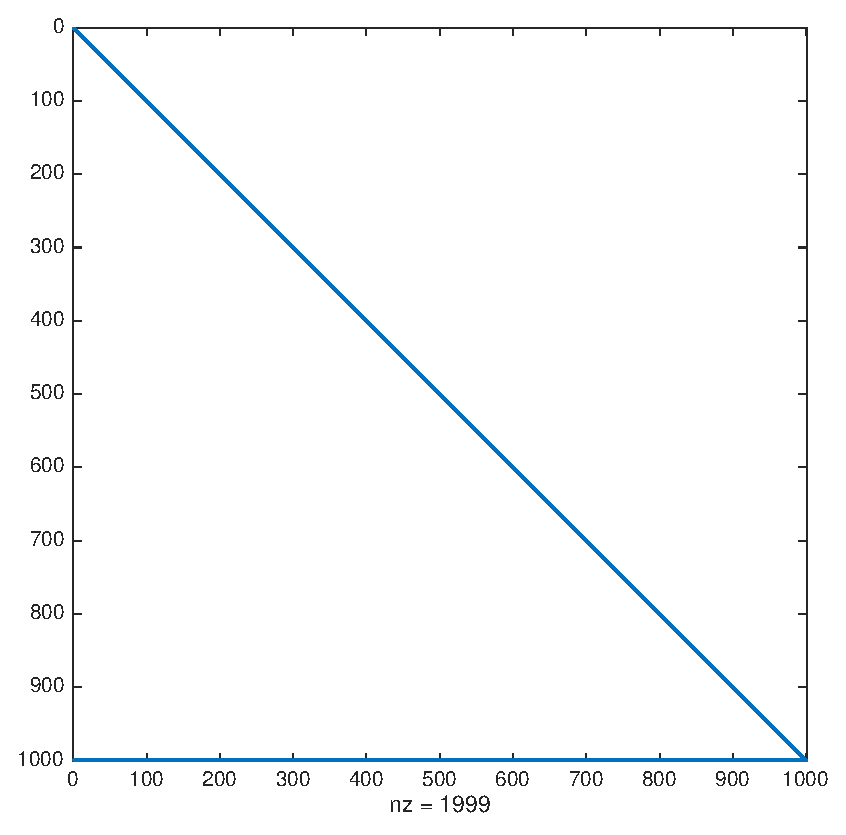
\includegraphics[scale=0.4]{s4/matlab/tildeL} 
       %\caption{Interpolation of $f$ using NCS \\ with $8+2$ points} 
       %\label{fig:q11_n8} 
     \end{subfigure}
     \begin{subfigure}[b]{0.5\linewidth}
       \centering
       \includegraphics[scale=0.4]{s4/matlab/tildeU} 
       %\caption{Interpolation of $f$ using NCS \\ with $8+2$ points} 
       %\label{fig:q11_n8} 
     \end{subfigure} 
     \caption{Structure des matrices $\tilde{L}$ (à gauche) et $\tilde{U}$ (à droite) telles que $\tilde{A} = \tilde{L} \tilde{U}$.}
     \label{fig:tildelu}
   \end{figure}  
   
   
   
   \item On peut noter que le nombre d'éléments non nuls passe de 500500 à 1999, donc il est 250 fois plus petit !
         Cette différence devient importante surtout quand on utilise un format de représentation des matrices creuses qui ne garde que les entrées non-nulles.
         Cela est fait en \textsc{MATLAB} à l'aide de la commande \texttt{sparse}.
         Normalement, si on travaille avec des matrices creuses et qu'on les converties au format creux, on gagne en memoire et en performance.
         Pour cet exemple, on peut voir la différence en tapant
         
\begin{verbatim}
sparseU = sparse(U);
sparseL = sparse(L);
sparse_tildeU = sparse(tildeU);
sparse_tildeL = sparse(tildeL);
whos
\end{verbatim} 

On trouve

\lstinputlisting{s4/matlab/out3.txt}


On voit que l'utilisation de la mémoire pour des matrices pleines est de 8 MB (en fait, comme les entrées sont des \texttt{double}, donc 8 Bytes, 8 * 1.000 * 1.000 = 8.000.000 Bytes = 8 MB).
Pour la première factorisation ($LU$), l'utilisation est même plus grande avec le format \texttt{sparse}, tandis que si on utilise la deuxième factorisation ($\tilde{L} \tilde{U}$), chaque facteur occupe moins de 40 KB, c'est-à-dire plus de 200 fois moins que dans le premier cas.


         
  
  Les figures de cet exercice sont obtenues avec le script \texttt{ex3.m}.

  \lstinputlisting{s4/matlab/ex3.m}





\end{enumerate}